\subsection{Equipos de referencia en el mercado}
Los generadores de funciones arbitrarias orientados a aplicaciones de laboratorio y enseñanza presentan un conjunto de características técnicas comunes que definen este segmento tecnológico. En términos generales, estos equipos ofrecen:

\begin{itemize}
	\item Rango de frecuencia senoidal típico entre 10 MHz a 30 MHz.
	\item Resolución vertical comprendida entre 12 y 14 bits.
	\item Impedancia de salida nominal de 50 $\Omega$.
	\item Amplitud máxima de hasta 20 Vpp en carga de alta impedancia.
	\item Offset DC ajustable.
	\item Control de fase relativo entre canales.
	\item Formas de onda convencionales (senoidal, cuadrada, triangular) y formas arbitrarias previamente cargadas.
\end{itemize}

Adicionalmente, suelen incorporar funcionalidades como barrido de frecuencia (sweep), generación por ráfagas (burst), modulación básica (AM/FM) y sincronización entre canales.

En cuanto a la interfaz de usuario, es habitual la presencia de pantalla gráfica, control rotativo incremental y conectividad mediante interfaces digitales como USB o LAN para control remoto.

El presente desarrollo se posiciona dentro de este rango tecnológico, tomando como referencia las prestaciones comúnmente ofrecidas en el segmento de media prestación.

%\subsubsection{UNIT-T Utg962e 60 Mhz:} Se trata de un generador de funciones arbitrario de 60 MHz. Posee algunas características que se destacan a continuación:
%
%\begin{itemize}
%	\item \textbf{Canales:} 2
%	\item \textbf{Frecuencia máxima:} 60\,MHz
%	\item \textbf{Tasa de muestreo (Sampling rate):} 200\,MS/s
%	\item \textbf{Resolución vertical:} 14\,bits
%	\item \textbf{Formas de onda:} Senoidal, cuadrada, pulso, rampa, ruido, DC y arbitraria
%	\item \textbf{Modos de barrido (Sweep):} Logarítmico y lineal
%	
%	\item \textbf{Características de frecuencia:}
%	
%	\begin{itemize}\renewcommand{\labelitemii}{$\bullet$}
%		\item Senoidal: $1\,\mu\text{Hz}$ -- $60\,\text{MHz}$
%		\item Cuadrada: $1\,\mu\text{Hz}$ -- $20\,\text{MHz}$
%		\item Rampa: $1\,\mu\text{Hz}$ -- $400\,\text{kHz}$
%		\item Pulso: $1\,\mu\text{Hz}$ -- $20\,\text{MHz}$
%		\item Arbitraria: $1\,\mu\text{Hz}$ -- $10\,\text{MHz}$
%		\item Resolución en frecuencia: $1\,\mu\text{Hz}$
%	\end{itemize}
%	
%	\item \textbf{Características de salida:}
%	\begin{itemize}\renewcommand{\labelitemii}{$\bullet$}
%		\item Impedancia: $50\,\Omega$ / High~Z
%		\item Rango de amplitud: $1\,\text{mVpp}$ -- $10\,\text{Vpp}$ (a $50\,\Omega$);\;
%		$2\,\text{mVpp}$ -- $20\,\text{Vpp}$ (High~Z)
%		\item Rango de offset DC (AC+DC): $\pm 5\,\text{V}$ (a $50\,\Omega$);\; $\pm 10\,\text{V}$ (High~Z)
%		\item Resolución de amplitud: $1\,\text{mV}$
%	\end{itemize}
%	
%	\item \textbf{Alimentación:} 100--240\,VAC, 50/60\,Hz
%	\item \textbf{Display:} 4.3'' TFT LCD (480$\times$272)
%\end{itemize}
%
%\begin{figure}[H]
%	\centering
%	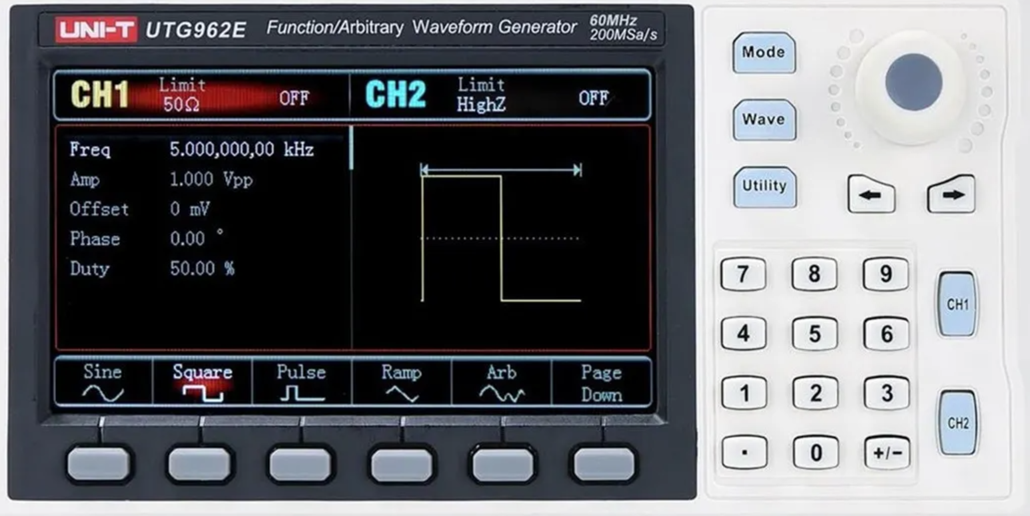
\includegraphics[width=0.7\linewidth]{Comparacion/img/unit-t}
%	\caption{Imagen ilustrativa del Generador de Funciones Arbitrarias de UNIT-T.}
%	\label{fig:unit-t}
%\end{figure}
%
%\subsubsection{OWON DGE2035:}
%Generador de funciones/arbitrario de \textbf{2 canales} con frecuencia máxima de \textbf{35\,MHz}. Sus características principales son:
%
%\begin{itemize}
%	\item \textbf{Canales:} 2
%	\item \textbf{Frecuencia máxima (salida):} 35\,MHz
%	\item \textbf{Tasa de muestreo (Sampling rate):} 125\,MSa/s
%	\item \textbf{Resolución vertical:} 14\,bits
%	\item \textbf{Longitud de forma arbitraria:} hasta 8K puntos
%	\item \textbf{Formas de onda:} senoidal, cuadrada, pulso, rampa y ruido; además incluye \textbf{150} formas arbitrarias predefinidas y permite forma arbitraria definida por el usuario
%	\item \textbf{Características de frecuencia (resolución en frecuencia: 1\,$\mu$Hz):}
%	\begin{itemize}\renewcommand{\labelitemii}{$\bullet$}
%		\item Senoidal: $1\,\mu\text{Hz}$ -- $35\,\text{MHz}$
%		\item Cuadrada: $1\,\mu\text{Hz}$ -- $15\,\text{MHz}$
%		\item Pulso: $1\,\mu\text{Hz}$ -- $15\,\text{MHz}$
%		\item Rampa: $1\,\mu\text{Hz}$ -- $1\,\text{MHz}$
%		\item Arbitraria: $1\,\mu\text{Hz}$ -- $10\,\text{MHz}$
%	\end{itemize}
%	\item \textbf{Modulación:} AM, FM, PM, FSK, Sweep y Burst
%	\item \textbf{Interfaz/Control:} USB Host; compatible con SCPI y LabVIEW
%	\item \textbf{Display:} TFT 3.6'' (480$\times$272)
%\end{itemize}
%
%\begin{figure}[H]
%	\centering
%	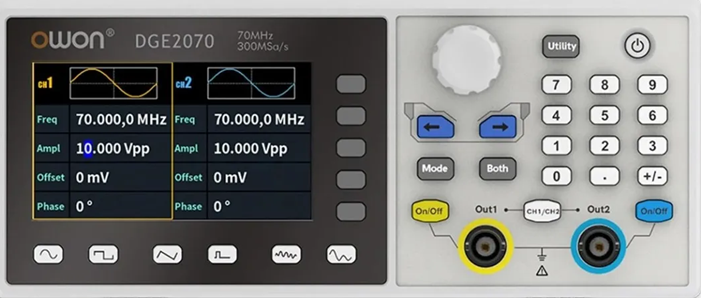
\includegraphics[width=0.7\linewidth]{Comparacion/img/owon}
%	\caption{Generador de Funciones Arbitrarias de la marca OWON.}
%	\label{fig:owon}
%\end{figure}
%
%\subsubsection{Generador DDS FeelElec FY6900-20M (20\,MHz):}
%Generador de funciones/arbitrario \textbf{de dos canales} basado en \textbf{DDS}. Especificaciones principales:
%
%\begin{itemize}
%	\item \textbf{Canales:} 2
%	\item \textbf{Tecnología:} DDS (Direct Digital Synthesizer)
%	\item \textbf{Tasa de muestreo (Sampling rate):} 250\,MSa/s
%	\item \textbf{Resolución vertical:} 14\,bits
%	\item \textbf{Longitud de forma arbitraria:} 8192 puntos (8K) \,$\times$\,14\,bits
%	\item \textbf{Resolución mínima de frecuencia:} 1\,$\mu$Hz
%	
%	\item \textbf{Rangos de frecuencia (modelo 20\,MHz):}
%	\begin{itemize}\renewcommand{\labelitemii}{$\bullet$}
%		\item Senoidal: 0--20\,MHz
%		\item Cuadrada: 0--15\,MHz
%		\item Triangular / Rampa: 0--10\,MHz
%		\item Pulso: 0--10\,MHz \;(\textbf{ancho mínimo de pulso:} 20\,ns)
%		\item Arbitraria: 0--10\,MHz
%	\end{itemize}
%	
%	\item \textbf{Formas de onda:} Seno, cuadrada, rectangular (duty ajustable), pulso, triangular/rampa,
%	diente de sierra, DC, ruido, ECG, y formas arbitrarias (predefinidas y definidas por el usuario)
%	
%	\item \textbf{Salida:}
%	\begin{itemize}\renewcommand{\labelitemii}{$\bullet$}
%		\item Impedancia de salida: 50\,$\Omega$ (típica, $\pm 10\%$)
%		\item Resolución de amplitud: 1\,mV
%		\item Rango de amplitud (Vpp) según frecuencia:
%		\begin{itemize}
%			\item $f \le 5\,\text{MHz}$: 1\,mVpp -- 24\,Vpp
%			\item $5\,\text{MHz} < f \le 10\,\text{MHz}$: 1\,mVpp -- 20\,Vpp
%			\item $10\,\text{MHz} < f \le 20\,\text{MHz}$: 1\,mVpp -- 10\,Vpp
%			\item $f > 20\,\text{MHz}$: 1\,mVpp -- 5\,Vpp
%		\end{itemize}
%	\end{itemize}
%	
%	\item \textbf{Offset DC:}
%	\begin{itemize}\renewcommand{\labelitemii}{$\bullet$}
%		\item Rango: $\pm 12$\,V (hasta 20\,MHz), $\pm 2.5$\,V (por encima de 20\,MHz)
%		\item Resolución: 1\,mV
%	\end{itemize}
%	
%	\item \textbf{Fase:} 0--359.99$^\circ$ \;(\textbf{resolución:} 0.01$^\circ$)
%	\item \textbf{Duty cycle (rectangular):} 0.01\%--99.99\% \;(\textbf{resolución:} 0.01\%)
%	\item \textbf{Modulación:} AM, FM, PM, ASK, FSK, PSK
%	\item \textbf{Sweep:} lineal y logarítmico (frecuencia, amplitud, offset y duty)
%\end{itemize}
%
%\begin{figure}[H]
%	\centering
%	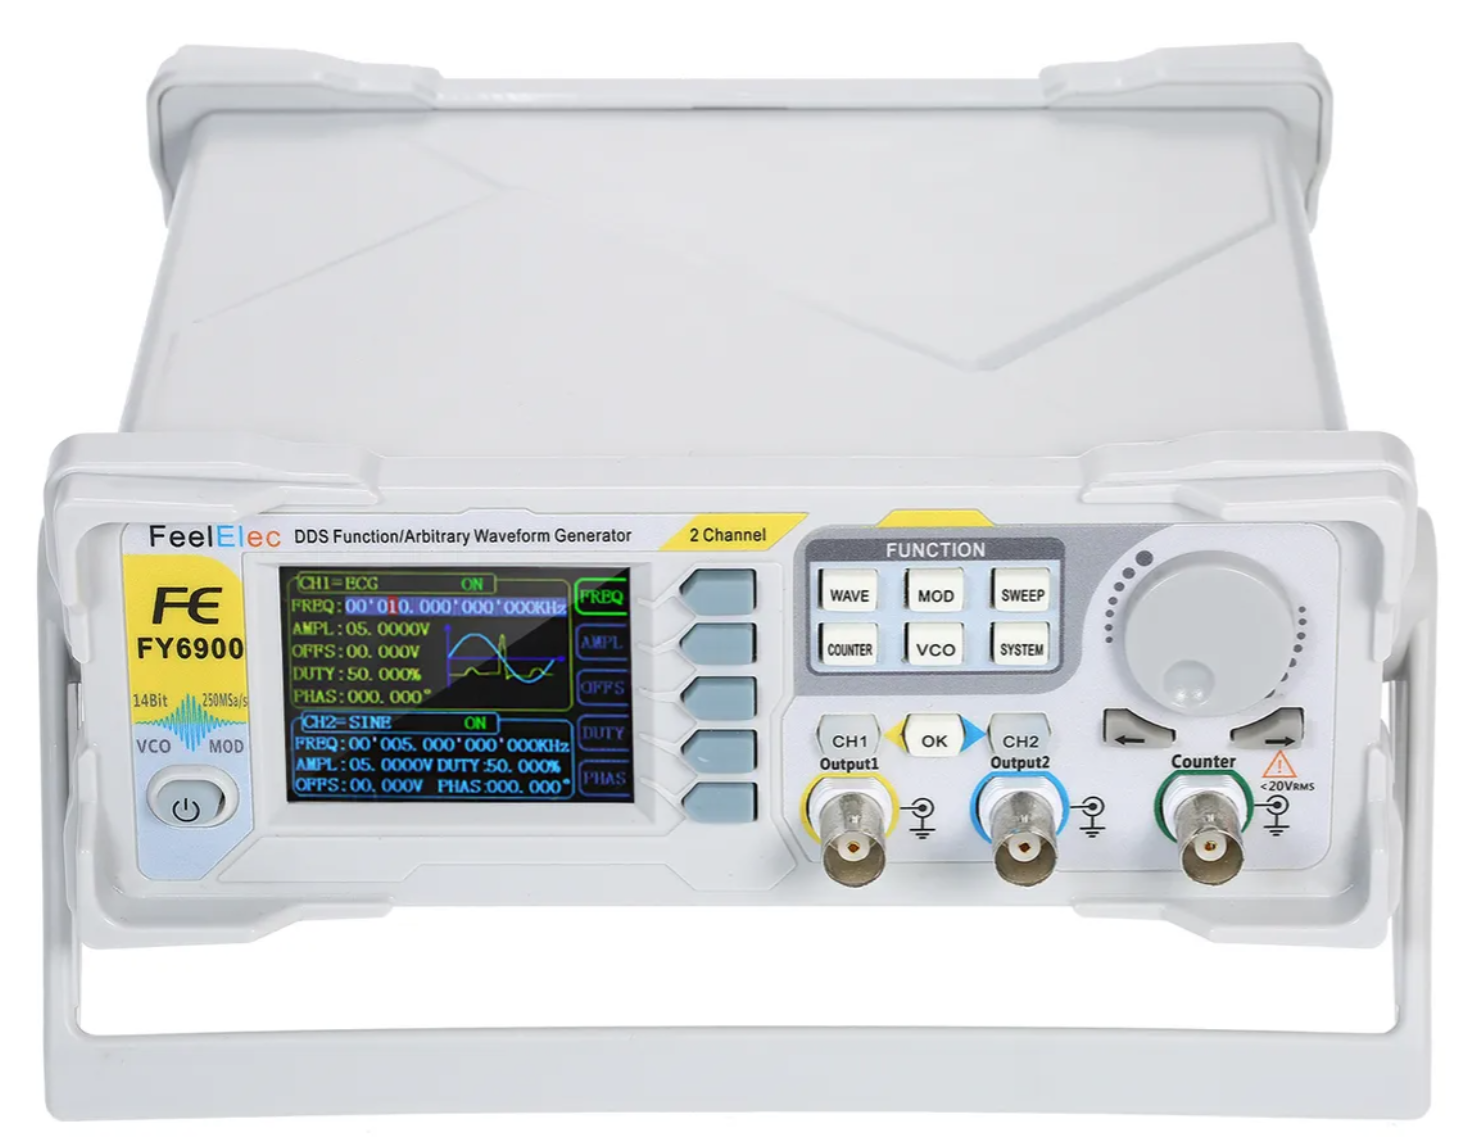
\includegraphics[width=0.7\linewidth]{Comparacion/img/Gaf-chino}
%	\caption{Generador de Funciones de marca FeelElec.}
%	\label{fig:gaf-chino}
%\end{figure}